\section{Implementazioni OpenMP}
\subsection{Introduzione}
Per parallelizzare l'algoritmo usando \emph{OpenMP} sono state realizzate alcune versioni in modo da valutare l'efficacia di diversi approcci o strumenti.
In particolare è risultato evidente che impostando la variabile d'ambiente \texttt{OMP\_PROC\_BIND=true} si ottengono risultati migliori sia dal punto di vista dell'efficienza, ma soprattutto da quello della \textbf{ripetibilità}: senza l'utilizzo della variabile esecuzioni successive dello stesso programma terminavano spesso in tempi molto diversi.

\subsection{Riduzione}
Analizzando il funzionamento dell'algoritmo si può dire che ad ogni iterazione viene aggiunto all'\emph{hull} il punto più esterno rispetto all'ultimo inserito $P_l$;
$P_a$ è più esterno di $P_b$ se la spezzata $P_lP_aP_b$ è orientata in senso orario.

È possibile quindi utilizzare il \textbf{pattern reduction} ad ogni iterazione per scegliere il punto più esterno, specificando la direttiva \texttt{reduce} di \emph{OpenMP}.\\
Per poter eseguire la \emph{reduction} su punti e per gestire il contesto necessario (per confrontare due punti è bisogna conoscere il punto precedente),
è stata dichiarato un operatore personalizzato con la direttiva \texttt{omp declare reduction}: esso lavora su una struttura dati apposita che contiene
un puntatore al punto da confrontare e uno al punto precedente\footnote{Il codice di questa prima versione è contenuto nel file \texttt{src/omp-reduction.c}}.

Già con questa soluzione è possibile ottenere un buon risultato, ma ci sono alcuni aspetti che si possono provare a migliorare.

\subsection{Pool di thread e \emph{First Touch}}
Si cerca quindi di evitare che il pool di thread venga ricreato ad ogni iterazione dell'algoritmo, quando si raggiunge la sezione \texttt{parallel for};
è possibile farlo includendo tutto il codice dell'algoritmo all'interno di un blocco \texttt{omp parallel}, al cui interno è presente il ciclo \texttt{omp for} per la ricerca del prossimo punto;
chiaramente in questo caso è necessario gestire adeguatamente le parti seriali (ad esempio l'aggiunta del punto al \emph{convex hull}).

Inoltre si è cercato di sfruttare il principio di \emph{First Touch}\footnote{https://software.intel.com/content/www/us/en/develop/articles/memory-allocation-and-first-touch.html} per velocizzare l'accesso alla memoria:
nelle architetture \emph{NUMA} ogni \emph{NUMANode} accede più velocemente alla propria memoria locale;
dato che è necessario considerare tutti i punti ad ogni iterazione, ogni thread può copiare la partizione di valori su cui lavorerà in un nuovo vettore
allocato nella memoria locale del \emph{NUMANode} su cui viene eseguito
(grazie alla variabile \texttt{OMP\_PROC\_BIND} i thread non dovrebbero venire spostati su core diversi).\\
Molti dei moderni sistemi operativi applicano inoltre la politica del \emph{First Touch}: le pagine di memoria allocata dal programma vengono istanziate solamente al momento della prima
scrittura, e vengono quindi posizionate nella memoria locale del \emph{NUMANode} thread che ha effettuato la scrittura.

Si utilizza quindi un ciclo \texttt{omp for schedule(static)} iniziale per copiare i punti in una nuova area di memoria, e un secondo ciclo con la stessa direttiva per eseguire la riduzione: in questo modo, dato che i due cicli vengono \emph{schedulati} nello stesso modo in fase di compilazione, i punti che vengono copiati da un thread sono gli stessi che verranno poi utilizzati dallo stesso thread.

Purtroppo questi tentativi in pratica non hanno portato alcun vantaggio, e anzi risultano in un leggero rallentamento, come mostrato nel confronto in figura \ref{fig:comparison}.

\subsection{Riduzione manuale}
Nella terza e ultima versione non viene più utilizzata la direttiva \texttt{omp for reduce}, ma la riduzione viene fatta manualmente accumulando i valori
ridotti da ogni thread all'interno di un vettore: i valori così ottenuti vengono poi ridotti in modo seriale da un singolo thread.\\
Ogni thread inoltre alloca un nuovo vettore in cui copia i punti che utilizzerà per la riduzione; questo sempre per cercare di utilizzare locale dei \emph{NUMANode}.
La copia viene effettuata solamente se il numero di punti utilizzato da ogni thread è superiore a $10\,000$ (valore scelto empiricamente):
se fosse inferiore il vantaggio ottenuto dalla località della memoria sarebbe annullato dal lavoro necessario alla copia.

Questa volta si ottiene un miglioramento delle prestazioni: di seguito sono mostrati quindi i grafici di \emph{speedup} ed efficienza relativi a questa soluzione

\begin{plot}
    \includeplot{speedup-omp-convex-hull}
    \caption{Speedup ottenuto realizzando manualmente la riduzione}
\end{plot}

È possibile notare come negli input più piccoli si ottenga uno speedup quasi inversamente proporzionale, probabilmente dovuto all'introduzione di un overhead troppo elevato rispetto alla dimensione dei dati da trattare.


\begin{plot}
    % \includeplot{omp-comparison}
    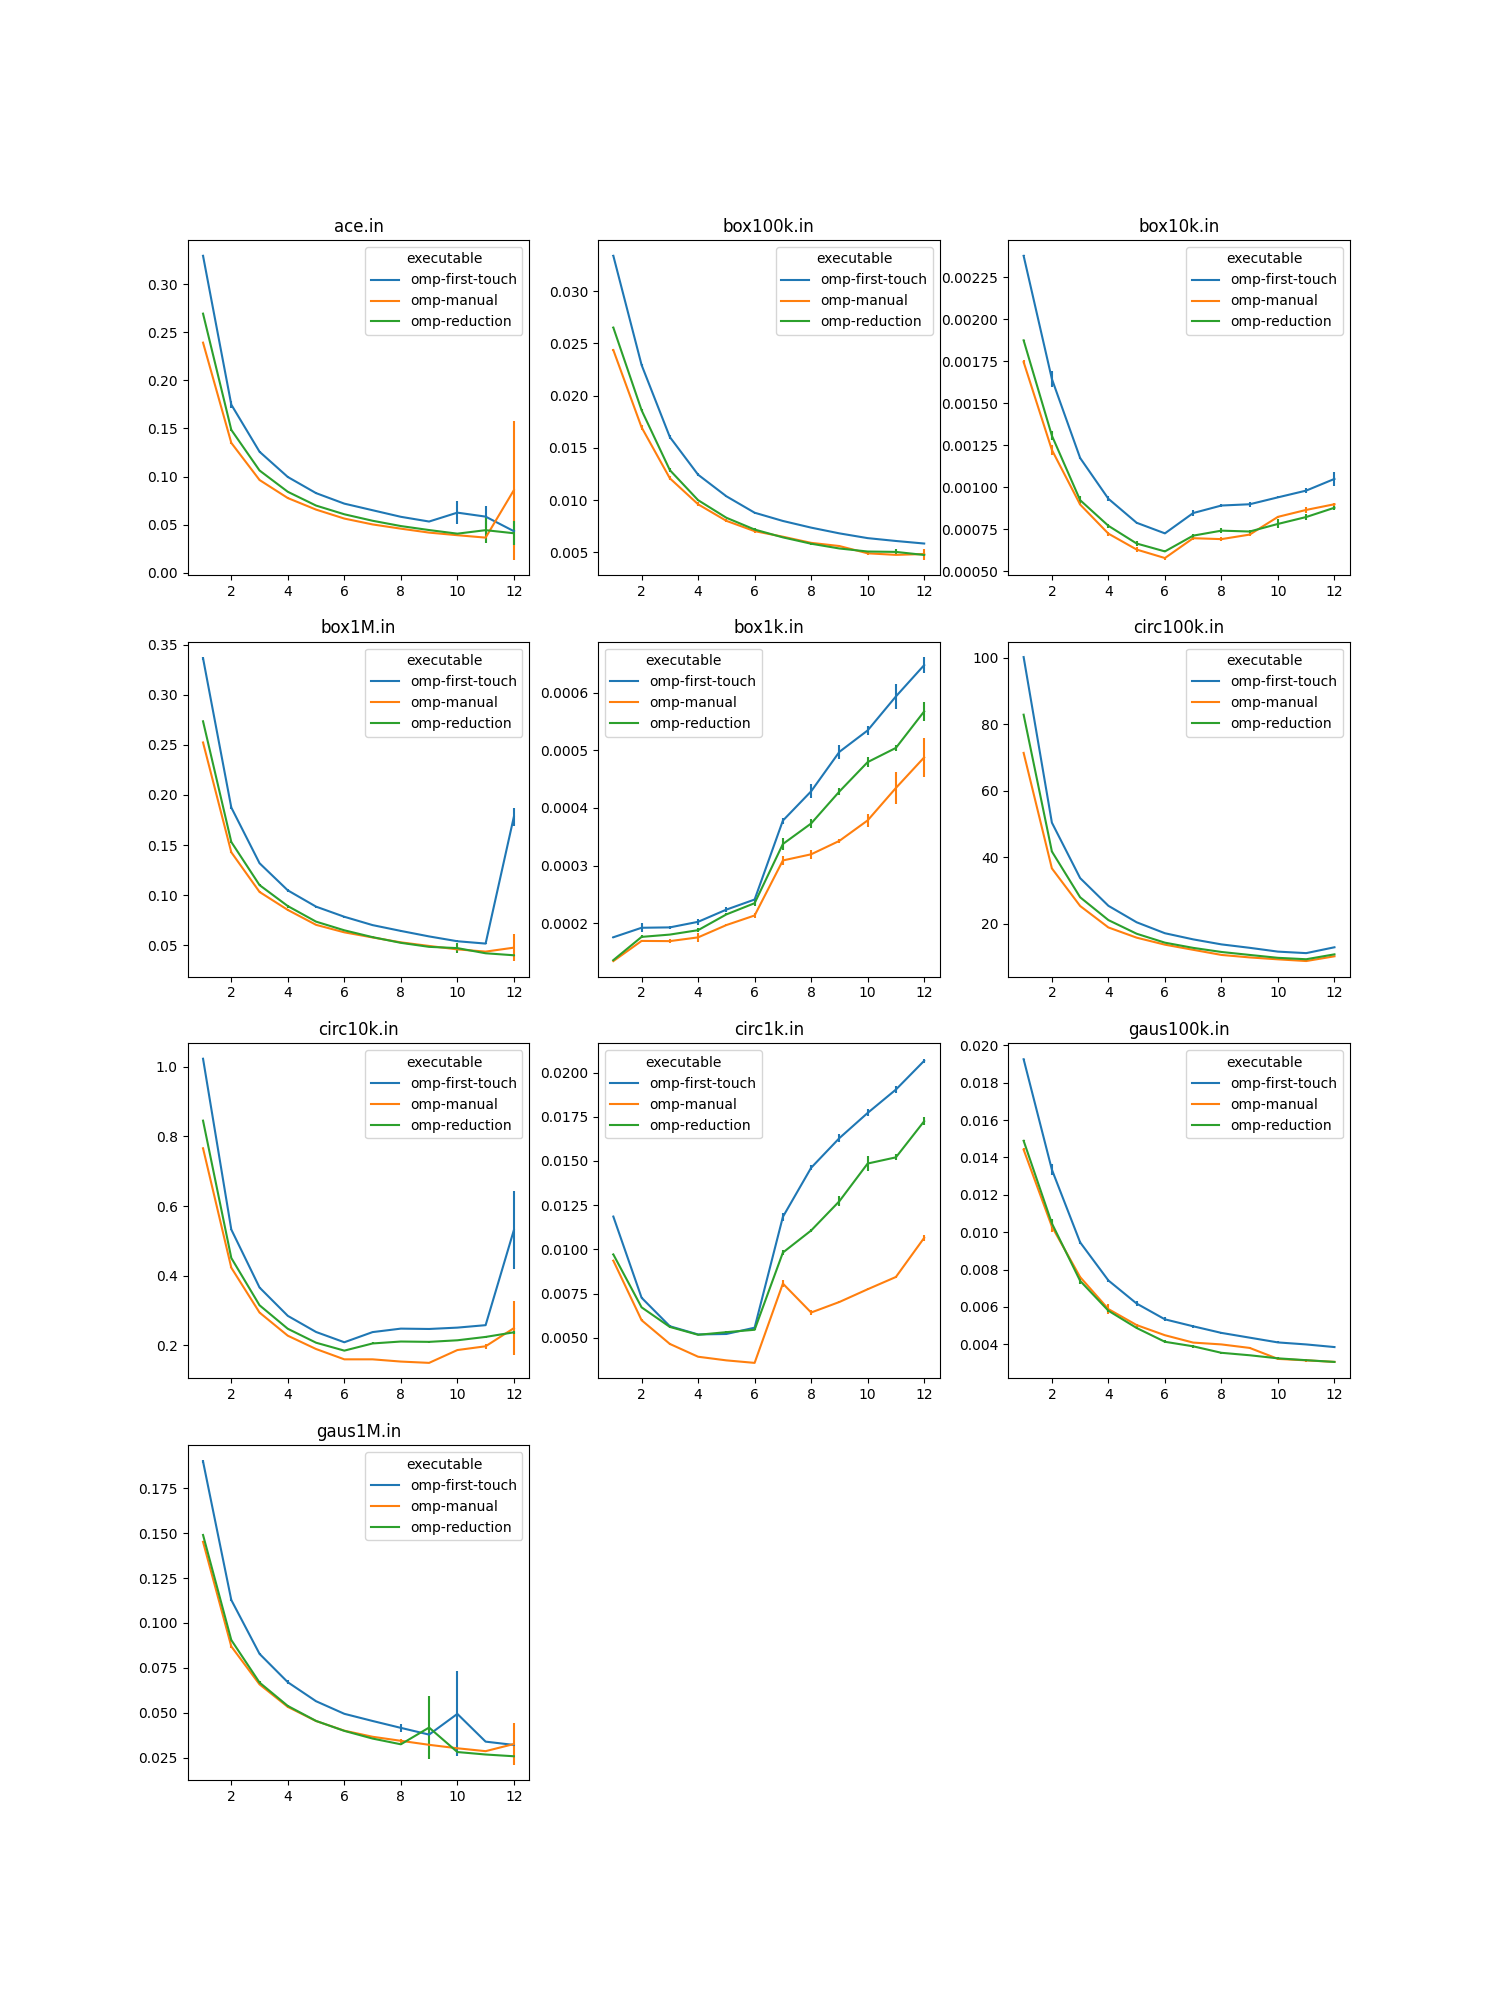
\includegraphics[width=\textwidth]{omp-comparison}
    \caption{TODO}
    \label{fig:comparison}
\end{plot}
